\subsection{Hemmelig kommunikation før internettet}
I dette afsnit vil vi kigge ind i hvordan man tidligere har brugt Kryptografi, altså i tiden inden internettets udbredelse, som skete i det sene 1980. \\
Dog for at skabe klarhed over begrebet kigger vi først på selve definitionen af Kryptografi og hvad dets endelige mening er. 
Kunsten at kryptografere betyder, at skjule information ved at transformere en mening ind i en forudbestemt algoritme.
Dette vil sige at kryptografering ikke bolt betyder at skjule, eller hemmeliggøre en støre mening, men næremere betyder det at transformere noget førhenværende forståeligt, til noget der kun kan forståes, ved brug af en bestemt metode.\cite{MeningOfCryptography}\\
Grundet denne definitionen, kan man også argumentere for, at alle de verdens forskellige sprogs bogstaver og tegn, enten har været, eller stadig er, en form for uforståelig kryptografi, og derfor skal vi kigge på det ældgamle Egypten, 1900 B.C. for at finde de ældste daterede tegn på, eller former for, Kryptografi.\cite{PastCryptography} Selv om man dog også kan diskutere hvorvidt der forefindes noget ældre, så som hulemændenes forskellige væg tegninger.
\begin{figure}[H]
    \centering
    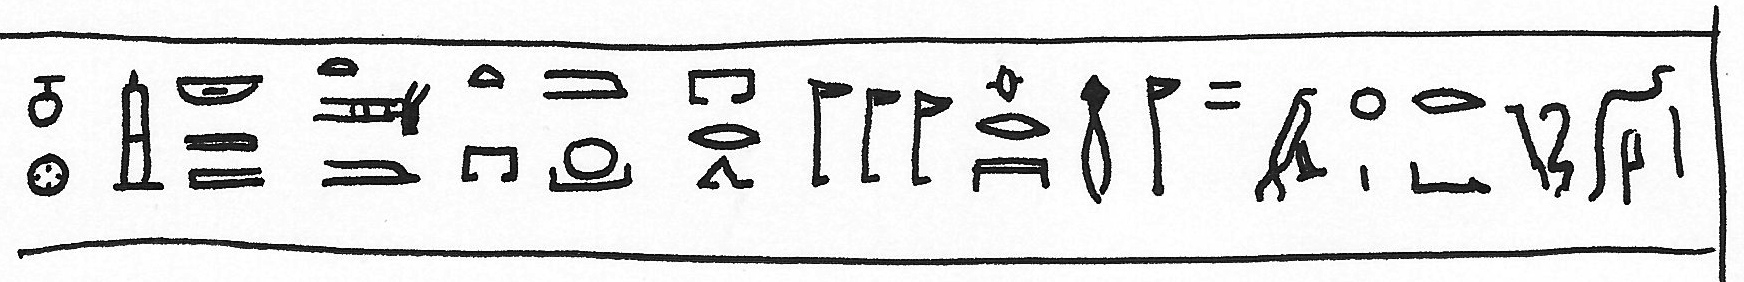
\includegraphics[width=0.8\textwidth, angle =0]{Projectdoc/egypten14.jpg}
    \caption{Egyptiske Hieroglyffer}
    \label{fig:hieroglyffer}
\end{figure}
\noindent
Disse hieroglyffer siges nemlig at være menneskets første form for tekst, og må derfor i begyndelsen ikke have været for alle at forstå. Dog som tiden udviklede sig, lærte det almene Egypten at tolke hieroglyffer, og denne første kryptografi, "De Egyptiske hieroglyffer [Se Figur: \ref{fig:hieroglyffer}]", blev til et anerkendt sprog.
Herefter er de næste former for Kryptografi selvfølgelig alle de andre sprog som efterhånden viste sig, og senere udbredte sig til det almene i de enkelte lande.\\
I takt med denne udbredelse viste der sig dog et nyt behov, behovet for at kunne skjule sine beskeder for andre, der også kunne læse eller skrive ens eget sprog. Den første løsningen på dette behov skal findes i årene omkring 500 B.C.\cite{PastCryptography} \\
\begin{figure}[H]
    \centering
    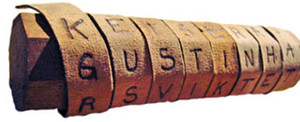
\includegraphics[scale=1.2]{Projectdoc/Problemanalyse/Illustrationer/Scytale.jpg}
    \caption{En Spartansk Scytale}
    \label{fig:scytale}
\end{figure}
\noindent
Da det stadig i denne tid kun var de færreste, der kunne læse og skrive, betød dette at de der faktisk kunne, reelt ikke havde den bedste forståelse for bogstavernes sammenhæng, og Spartanerne kunne derfor opfinde en af de første former for kryptering, "Den Spartanske Scytale [Se Figur:\ref{fig:scytale}]". Denne Spartanske Scytale var en cylinder, hvorom man viklede noget at skrive på, herefter skrev man sin besked på de enkelte sider, og således når man fjernede cylinderen kunne man ikke forstå sammenhængen før man havde en ligeledes størrelsesmæssig cylinder. Denne kryptering ville dog i dag ikke være særlig svær at dekryptere, og kendes også i flere former under bogstavs transponering.\\
Den næste daterede form for kryptering findes allerede små 500 år efter, i det gamle Rom, regeret under Julius Caesar, og siges faktisk også at være opfundet af Julius Caesar ham selv.\cite{PastCryptography}\\ 
Det romerske militær havde brug for at skjule deres strategiske beskeder for fjenden, som ofte fangede de Romerske budbringer, i forsøget på at danne et militærisk modtræk. Ceasar opfandt derfor, den største af de nu tids kendte kryptografi's metoder, kaldet bogstavs substitution eller "A-K Koden".\\
A-K Koden går i alt sin simpelhed ud på, at man flytter alfabetet en vis grad, f.eks. i A-K ville "ABCD" skrives "KLMN", eller i A-S ville "ABCD" skrives "STUV".\cite{TheSecretLanguage}
Som førnævnt er denne bogstavs substitution den mest udbredte og kendte kryptografi's metode, og er derfor også den mest udviklede. A-K Koden findes nemlig også i et utal af andre former.\\ 
F.eks. i formen af "Det hemmelig kodeords A-K", der udføres ved at først vælge et kodeord, "KODEORD", hvorefter kodeordets bogstaver flyttes til starten af alfabetet for tilsidst af fortsættes resten af alfabetet, derfor ville "ABCDEFGHIJKLMNO" skrives "KODEORDABCFGHIJ", således at "HEJ" ville skrives "AOC". \cite{TheSecretLanguage}
Andre former af A-K Koden kunne være "Alberti-Vigeneres Cipher" opfundet i midt 1400 tallet, "The Vingenere Cipher" fra 1500'erne, eller Jefferson's Wheel Cipher fra det sene 1700,\cite{PastCryptography} der alle som Caesar's koncept, fungere ved udbytning af bokstavernes rækkefølge, men dog i de nævnte også ved hjælp af et værktøj, som ved Den Spartanske Scytale.



--------------- NOTER --------------\\
Som to nyere kan nævnes WWII's kryptografi maskiner, Morsing, og
Allernyest The Da Pinchi Code, (Tyvene idag bruger denne kode.) the hobo code